\section{Lecture 9: Unit Impulse Response of the RC circuit}


\subsection{Taking the derivative of the input signal for an LSI system}
Let \textbf{S} be a Linear Shift-Invariant system, and let $y(t)$ be the output corresponding to an input signal $x(t)$.\\
\indent Because of the Shift invariance of the \textbf{S}, $x(t+\Delta)$ will produce an output of $y(t+\Delta)$
\begin{figure}[H]
	\centering
	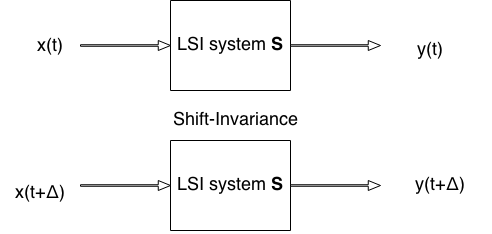
\includegraphics[width=0.6\textwidth]{shift_inv_1.png}
	\caption{Shift-invariance}
\end{figure}
\indent Homogeneity implies that $-x(t)$ will result in an output of $-y(t)$. And thus using additivity, an input of $x(t+\Delta)-x(t)$ will produce an output of $y(t+\Delta)-y(t)$.
\begin{figure}[H]
	\centering
	
\includegraphics[width=0.6\textwidth]{ad_hom.png}
	\caption{Additivity and Homogeneity}
\end{figure}
\indent Invoking homogeneity with a scaling of $\frac{1}{\Delta}$, and taking the limit $\Delta\rightarrow0$, we obtain the result that the derivative of $x(t)$ produces the derivative of $y(t)$, as the output.
\begin{figure}[H]
	\centering
	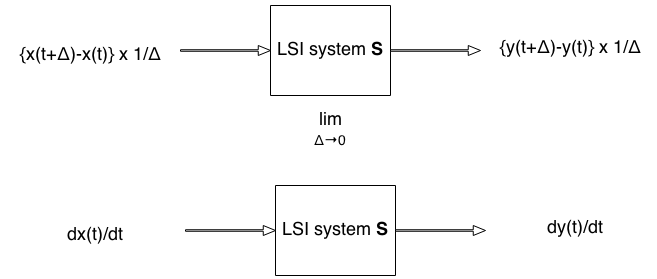
\includegraphics[width=0.8\textwidth]{derixt_deriyt.png}
	\caption{Scaling by $\Delta$ followed by taking the limit $\Delta\rightarrow 0$}
\end{figure}


\subsubsection{Impulse response of the RC circuit}
Now we can finally obtain the impulse response of the RC circuit. To do this, we need to apply the result of the previous section to the the unit step response of the RC circuit. As discussed previously, the unit step response of the RC circuit is the function $s(t)=(1-e^{-\frac{t}{\tau}})u(t)$.\\
\indent Now, since the RC circuit is an LSI system, the derivative of $u(t)$ should produce the derivative of $s(t)$! But we already know that the derivative of the unit step function is the unit impulse. Thus the unit impulse response is nothing but the derivative of the unit step response $s(t)$!\\
Using the product rule for differentiation, we get
\begin{eqnarray*}
\frac{ds(t)}{dt} &=& u(t)\Big\{\frac{d}{dt}(1-e^{-\frac{t}{\tau}})\Big\} + (1-e^{-\frac{t}{\tau}})\frac{du(t)}{dt}\\
&=& \frac{1}{\tau}e^{-\frac{t}{\tau}}u(t)+(1-e^{-\frac{t}{\tau}})\delta(t)
\end{eqnarray*}
\indent Now note that the second term in the expression is the delta function multiplied by another function. But $f(t)\delta(t)=f(0)\delta(t)$. The second term in the above equation vanishes, since f(0)=0 in this case. Thus we obtain,
$$\frac{ds(t)}{dt}=\frac{1}{\tau}e^{-\frac{t}{\tau}}u(t)$$
This is the formula for the Impulse Response of an RC circuit.
\subsubsection{Interpretation of the RC unit Impulse Response}
We can try to understand how this result makes sense physically.\\
\indent Applying a unit impulse voltage across the RC voltage is like suddenly pumping in an amount of charge into the circuit. Let us use the $\delta_\Delta$ function instead of the the unit impulse, since it is easier to interpret applying a finite voltage $\frac{1}{\Delta}$ over a finite time $\Delta$. Since the voltage across a capacitor does not behave in an `impulsive' manner, this sudden jump in the voltage at $t=0$ is sustained by the resistor R, setting up a current:
$$I=\frac{1}{\Delta}.\frac{1}{R}$$
Now, at the same time, the same current flows through the Capacitor, and integrating this current gives us the capacitor charge:
$$\textrm{Capacitor Charge}=\Delta .\frac{1}{\Delta} .\frac{1}{R}$$
Resulting in a voltage across the Capacitor (at time $t=0$ ):
\begin{eqnarray*}
\textrm{Capacitor Voltage at time t=0}&=&\Delta .\frac{1}{\Delta} .\frac{1}{R} .\frac{1}{C} \\
&=&\frac{1}{RC}\\
&=& \frac{1}{\tau}
\end{eqnarray*}
\indent Since there is no applied voltage across the circuit after $t=0$, the capacitor simply discharges exponentially, thus giving us :
\[
\textrm{Capacitor voltage, i.e. output voltage}=\frac{1}{\tau}e^{-\frac{t}{\tau}}u(t) 
\]
%\tag{3.1.1a,b}
	